{
\newcommand{\nodeA}{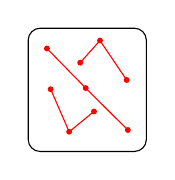
\begin{tikzpicture}[scale=1*0.5, every node/.style={scale=1}]
    \def\xscale{0.5} % Horizontal scale factor
    \def\yscale{0.5} % Vertical scale factor
    \def\spnt{0.075} % Size of smaller points
    \def\lpnt{0.125} % Size of larger points
    \def\roundscale{0.5} % The rounding factor
    \draw[rounded corners=2ex*\roundscale] (0,0) rectangle (6.0*\xscale,6.26*\yscale);
    \fill[red] (2.64*\xscale, 4.51*\yscale) circle (\spnt);
    \fill[red] (3.645242338035261*\xscale, 5.634518213709113*\yscale) circle (\spnt);
    \fill[red] (5.0*\xscale, 3.63*\yscale) circle (\spnt);
    \draw[red] (2.64*\xscale, 4.51*\yscale) -- (3.645242338035261*\xscale,5.634518213709113*\yscale) -- (5.0*\xscale,3.63*\yscale);
    \fill[red] (1.14*\xscale, 3.16*\yscale) circle (\spnt);
    \fill[red] (2.08*\xscale, 1.0*\yscale) circle (\spnt);
    \fill[red] (3.34*\xscale, 2.03*\yscale) circle (\spnt);
    \draw[red] (1.14*\xscale, 3.16*\yscale) -- (2.08*\xscale,1.0*\yscale) -- (3.34*\xscale,2.03*\yscale);
    \fill[red] (0.95*\xscale, 5.23*\yscale) circle (\spnt);
    \fill[red] (2.92*\xscale, 3.22*\yscale) circle (\spnt);
    \fill[red] (5.06*\xscale, 1.09*\yscale) circle (\spnt);
    \draw[red] (0.95*\xscale, 5.23*\yscale) -- (2.92*\xscale,3.22*\yscale) -- (5.06*\xscale,1.09*\yscale);
\end{tikzpicture}}
\newcommand{\nodeB}{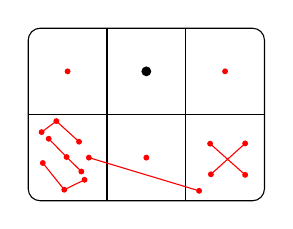
\begin{tikzpicture}[scale=1*0.5, every node/.style={scale=1}]
    \def\xscale{1.0} % Horizontal scale factor
    \def\yscale{0.7} % Vertical scale factor
    \def\spnt{0.075} % Size of smaller points
    \def\lpnt{0.125} % Size of larger points
    \def\roundscale{0.5} % The rounding factor
    \fill[red] (1.0*\xscale,4.695*\yscale) circle (\spnt);
    \fill[red] (3.0*\xscale,1.565*\yscale) circle (\spnt);
    \fill[red] (5.0*\xscale,4.695*\yscale) circle (\spnt);
    \draw[rounded corners=2ex*\roundscale] (0,0) rectangle (6.0*\xscale,6.26*\yscale);
    \draw (2.0*\xscale, 6.26*\yscale) -- (2.0*\xscale, 0);
    \draw (4.0*\xscale, 6.26*\yscale) -- (4.0*\xscale, 0);
    \draw (0, 3.13*\yscale) -- (6.0*\xscale, 3.13*\yscale);
    \fill[red] (4.64*\xscale, 0.96*\yscale) circle (\spnt);
    \fill[red] (5.51*\xscale, 2.08*\yscale) circle (\spnt);
    \draw[red] (4.64*\xscale, 0.96*\yscale) -- (5.51*\xscale,2.08*\yscale);
    \fill[red] (1.54*\xscale, 1.56500*\yscale) circle (\spnt);
    \fill[red] (4.34*\xscale, 0.36*\yscale) circle (\spnt);
    \draw[red] (1.54*\xscale, 1.56500*\yscale) -- (4.34*\xscale,0.36*\yscale);
    \fill[red] (4.62*\xscale, 2.07*\yscale) circle (\spnt);
    \fill[red] (5.51*\xscale, 0.94*\yscale) circle (\spnt);
    \draw[red] (4.62*\xscale, 2.07*\yscale) -- (5.51*\xscale,0.94*\yscale);
    \fill[red] (0.34*\xscale, 2.49*\yscale) circle (\spnt);
    \fill[red] (0.7137700370786788*\xscale, 2.8907811732342776*\yscale) circle (\spnt);
    \fill[red] (1.29*\xscale, 2.1410793034814266*\yscale) circle (\spnt);
    \draw[red] (0.34*\xscale, 2.49*\yscale) -- (0.7137700370786788*\xscale,2.8907811732342776*\yscale) -- (1.29*\xscale,2.1410793034814266*\yscale);
    \fill[red] (0.37*\xscale, 1.37*\yscale) circle (\spnt);
    \fill[red] (0.9155476869638484*\xscale, 0.3994524095796065*\yscale) circle (\spnt);
    \fill[red] (1.43*\xscale, 0.76*\yscale) circle (\spnt);
    \draw[red] (0.37*\xscale, 1.37*\yscale) -- (0.9155476869638484*\xscale,0.3994524095796065*\yscale) -- (1.43*\xscale,0.76*\yscale);
    \fill[red] (0.52*\xscale, 2.25*\yscale) circle (\spnt);
    \fill[red] (0.974077815720099*\xscale, 1.5866958340474693*\yscale) circle (\spnt);
    \fill[red] (1.35*\xscale, 1.06*\yscale) circle (\spnt);
    \draw[red] (0.52*\xscale, 2.25*\yscale) -- (0.974077815720099*\xscale,1.5866958340474693*\yscale) -- (1.35*\xscale,1.06*\yscale);
    \fill (3*\xscale,4.69500*\yscale) circle (\lpnt);
\end{tikzpicture}}
\newcommand{\nodeD}{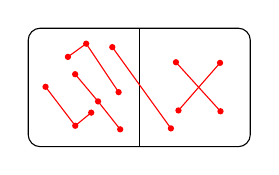
\begin{tikzpicture}[scale=0.4, every node/.style={scale=1}]
        \def\xscale{1.0} % Horizontal scale factor
        \def\yscale{1.0} % Vertical scale factor
        \def\spnt{0.1} % Size of smaller points
        \def\lpnt{0.125} % Size of larger points
        \def\roundscale{0.5} % The rounding factor
        \draw[rounded corners=2ex*\roundscale] (0,0) rectangle (7.05*\xscale,3.76*\yscale);
        \draw (3.525*\xscale, 3.76*\yscale) -- (3.525*\xscale, 0);
        \fill[red] (4.77*\xscale, 1.15*\yscale) circle (\spnt);
        \fill[red] (6.09*\xscale, 2.66*\yscale) circle (\spnt);
        \draw[red] (4.77*\xscale, 1.15*\yscale) -- (6.09*\xscale,2.66*\yscale);
        \fill[red] (2.67*\xscale, 3.16*\yscale) circle (\spnt);
        \fill[red] (4.53*\xscale, 0.58*\yscale) circle (\spnt);
        \draw[red] (2.67*\xscale, 3.16*\yscale) -- (4.53*\xscale,0.58*\yscale);
        \fill[red] (4.69*\xscale, 2.68*\yscale) circle (\spnt);
        \fill[red] (6.103901218159451*\xscale, 1.1230608594818354*\yscale) circle (\spnt);
        \draw[red] (4.69*\xscale, 2.68*\yscale) -- (6.103901218159451*\xscale,1.1230608594818354*\yscale);
        \fill[red] (1.26*\xscale, 2.85*\yscale) circle (\spnt);
        \fill[red] (1.84*\xscale, 3.27*\yscale) circle (\spnt);
        \fill[red] (2.87*\xscale, 1.73*\yscale) circle (\spnt);
        \draw[red] (1.26*\xscale, 2.85*\yscale) -- (1.84*\xscale,3.27*\yscale) -- (2.87*\xscale,1.73*\yscale);
        \fill[red] (0.55*\xscale, 1.9*\yscale) circle (\spnt);
        \fill[red] (1.4930670970674682*\xscale, 0.6636520415041379*\yscale) circle (\spnt);
        \fill[red] (2.0*\xscale, 1.08*\yscale) circle (\spnt);
        \draw[red] (0.55*\xscale, 1.9*\yscale) -- (1.4930670970674682*\xscale,0.6636520415041379*\yscale) -- (2.0*\xscale,1.08*\yscale);
        \fill[red] (1.49*\xscale, 2.3*\yscale) circle (\spnt);
        \fill[red] (2.2169083602620874*\xscale, 1.4365892987622655*\yscale) circle (\spnt);
        \fill[red] (2.92*\xscale, 0.55*\yscale) circle (\spnt);
        \draw[red] (1.49*\xscale, 2.3*\yscale) -- (2.2169083602620874*\xscale,1.4365892987622655*\yscale) -- (2.92*\xscale,0.55*\yscale);
\end{tikzpicture}}
\begin{tikzpicture}
\fill[opacity=0] (-0.8,-1.2) rectangle (9.1,2.2);
\end{tikzpicture}
\begin{tikzpicture}[overlay,xshift=-9.25cm,yshift=1.15cm]
\draw<2-> (0,1) node {\tiny $1,1,2,3,5,\ldots$};
\node<2-> (a) at (0,0) {\nodeA};
\draw<3-> (3.5,2.25) node {\tiny $0,1,2,3,5,\ldots$};
\node<3-> (b) at (3.5,1) {\nodeB};
\node<3-> (c) at (3.5,-1)  {$\varepsilon$};
\node<4-> (e) at (7.5,2)  {\tikz{\fill (0,0) circle (0.1);}};
\draw<4-> (7.5,1) node {\tiny $1,2,3,5,8,\ldots$};
\node<4-> (d) at (7.5,0)  {\nodeD};

\draw<3-> (a) -- (b);
\draw<3-> (a) -- (c);
\draw<4-> (b) -- (d);
\draw<4-> (b) -- (e);

\draw<5->[orange!70] (6,-0.85) rectangle (9,0.85);
\end{tikzpicture}
}